\section{Background}\label{sect:back}

\subsection{Conventions}

We use $[m]$ to denote the set $\{1, \dots, m\}$. By $\binom{[m]}{k}$ we mean the set of subsets of $[m]$ of size $k$. For $l \in [m]$, using the notation of \cite{ops}, we use $<_{l}$ to denote the cyclically shifted order on $[m]$ given by \[l <_{l} l+1 <_{l} < \dots <_{l} m-1 <_{l} m <_{l} 1 <_{l} \dots <_{l} l-1 .\] For $r \geqslant 3$, $a_{1} < \dots < a_{r}$ is a \emph{cyclic ordering} if there is an $l \in [n + 2d + 1]$ such that $a_{1} <_{l} \dots <_{l} a_{r}$.

Throughout this paper, we will often need to change the ordering on $[m]$ to $<_{l}$ for some $l$. We will usually do this tacitly, rather than explicitly writing $<_{l}$ in place of $<$. Similarly, we will usually be tacitly using arithmetic modulo $n + 2d + 1$, where this will be the number of vertices of our cyclic polytope. Hence, we shall write things like $j = i - 1$, when we mean $j \equiv i - 1 \pmod{n + 2d + 1}$. Our convention here will also be that our equivalence-class representatives for arithmetic modulo $n + 2d + 1$ will be $[n + 2d + 1]$ rather than $\{0, 1, \dots, n + 2d\}$. This is because we shall label the vertices of our cyclic polytope by $[n + 2d + 1]$.

Finally, given a tuple $A \in [m]^{k + 1}$, we will denote the elements of $A$ by $(a_{0}, a_{1}, \dots, a_{k})$ where $a_{0} <_{l} a_{1} <_{l} \dots <_{l} a_{k}$ in a cyclically shifted order to be determined by the context. By default this will be the usual order on $[m]$. Because we wish sometimes to change this order, we are also tacitly identifying tuples which are the same up to cyclically shifted reordering. The same applies to other letters of the alphabet: the upper case letter denotes the tuple; the lower case letter is used for the entries, which are ordered according to their index, which starts from 0. For example, if we write $A = (1, 3, 5)$, then we have $a_{0} = 1$, $a_{1} = 3$, and $a_{2} = 5$. If we changed the cyclic ordering from $<_{1}$ to $<_{3}$, then we would have $A = (3, 5, 1)$ with $a_{0} = 3$, $a_{1} = 5$, and $a_{2} = 1$.

\subsection{Triangulations of cyclic polytopes}\label{sect:back:cyc}

Cyclic polytopes should be thought of as higher-dimensional analogues of convex polygons. General introductions to this class of polytopes can be found in \cite[Lecture 0]{ziegler}, \cite[4.7]{gruenbaum}, \cite[Section 6.1]{lrs} and \cite[Chapter VI]{bar}. Let $n \geqslant 0$ and $\delta \geqslant 1$ and consider the curve defined by $p_{t}=(t, t^{2}, \dots , t^{\delta}) \subset \mathbb{R}^{\delta}$ for $t \in \mathbb{R}$, which is known as the \emph{moment curve}. Choose $t_{1}, t_{2}, \dots , t_{n + \delta + 1} \in \mathbb{R}$ such that $t_{1} < t_{2} < \dots < t_{n + \delta + 1}$. The convex hull $\conv\{ p_{t_{1}}, p_{t_{2}}, \dots , p_{t_{n + \delta + 1}} \}$ is a \emph{cyclic polytope} $C(n + \delta + 1, \delta)$. A (\emph{geometric}) \emph{triangulation} of a cyclic polytope $C(n + \delta + 1, \delta)$ is a collection of (geometric) $\delta$-simplices whose interiors are pairwise disjoint and whose union is $C(n + \delta + 1, \delta)$.

A \emph{facet} of $C(n + \delta + 1, \delta)$ is a face of codimension one. A \emph{circuit} of a cyclic polytope $C(n + \delta + 1, \delta)$ is a pair, $(Z_{+}, Z_{-})$, of sets of vertices of $C(n + \delta + 1,\delta)$ which are inclusion-minimal with respect to the property $\mathrm{conv}(Z_{+}) \cap \mathrm{conv}(Z_{-}) \neq \emptyset$, in the sense that if $Z'_{+} \subseteq Z_{+}$ and $Z'_{-} \subseteq Z_{-}$ with $\mathrm{conv}(Z'_{+}) \cap \mathrm{conv}(Z'_{-}) \neq \emptyset$, then $Z'_{+} = Z_{+}$ and $Z'_{-} = Z_{-}$.

The circuits and facets of a cyclic polytope are independent of its particular geometric realisation given by the choice of points on the moment curve, by \cite{gale,breen}. This implies that whether or not a collection of ordered $(\delta + 1)$-tuples of $[n + \delta + 1]$ forms a triangulation of $C(n + \delta + 1, \delta)$ is likewise independent of the particular geometric realisation. Hence, in this paper we primarily consider triangulations combinatorially: a \emph{combinatorial triangulation} of $C(n + \delta + 1, \delta)$ is a collection of ordered $(\delta + 1)$-tuples with entries in $[n + \delta + 1]$ which gives a geometric triangulation of $C(n + \delta + 1, \delta)$. Unless otherwise specified, when we write `triangulation' we mean a combinatorial triangulation. Likewise, if we say that $A$ is a $k$-simplex, we mean that $A$ is an ordered $(k + 1)$-tuple with entries in $[n + \delta + 1]$. We write $|A|$ to denote the geometric realisation of $A$ as a geometric simplex which is the convex hull of $k + 1$ points on the moment~curve. 

In this paper we are exclusively interested in triangulations of even-dimensional cyclic polytopes. These were given an elegant combinatorial description in \cite{ot}, which we now explain. This combinatorial description was in turn used to connect triangulations of even-dimensional cyclic polytopes to representation theory of algebras. We will sometimes comment on these connections, but this paper does not require the reader to be familiar with representation theory.

A $d$-simplex of a triangulation of $C(n + 2d + 1, 2d)$ is \emph{internal} if it does not lie within a facet of $C(n + 2d + 1, 2d)$. It is clear that a triangulation of a convex polygon is determined by the arcs of the triangulation; similarly, a triangulation of $C(n + 2d + 1,2d)$ is determined by the internal $d$-simplices of the triangulation, by a theorem of Dey \cite{dey}. For brevity, we refer to an internal $d$-simplex of a triangulation $\mathcal{T}$ of $C(n + 2d + 1, 2d)$ as a \emph{$d$-arc} of $\mathcal{T}$. We write $\darcs{\mathcal{T}}$ for the set of $d$-arcs of $\mathcal{T}$. We say that a $(d + 1)$-simplex of $\mathcal{T}$ is \emph{interior} if all of its facets are $d$-arcs.

In order to recall the description of the triangulations of $C(n + 2d + 1,2d)$ from \cite{ot}, and for use later in the paper, we denote the following sets.
\begin{align*}
\derset{n + 2d + 1}{d} &= \set{(a_{0},\dots,a_{d}) \in \mathbb{Z}^{d+1} \st \parbox{5.5cm}{\begin{center}$\forall i \in \{0, 1, \dots ,d - 1\}, a_{i + 1} \geqslant a_{i} + 2 $\\  and  $a_{d} + 2 \leqslant a_{0} + n + 2d + 1$\end{center}}}; \\
\nonconsec{n + 2d + 1}{d} &= \derset{n + 2d + 1}{d} \cap [n + 2d + 1]^{d + 1}.
\end{align*}

\begin{rema}
Algebraically, $\derset{n + 2d + 1}{d}$ labels the $d$-cluster-tilting subcategory of the derived category of $A_{n}^{d}$, whilst $\nonconsec{n + 2d + 1}{d}$ labels its cluster category \cite{ot}. Here $A_{n}^{d}$ is the higher Auslander algebra of type~$A$; see \cite{iy-clus}.
\end{rema}

A $d$-simplex $A \in [n + 2d + 1]^{d + 1}$ is a $d$-arc in $C(n + 2d + 1, 2d)$ if and only if $A \in \nonconsec{n + 2d + 1}{d}$. A $d$-simplex $A$ and a $d$-simplex $B$ are \emph{intertwining} if \[ a_{0} < b_{0} < a_{1} < b_{1} < \dots < a_{d} < b_{d}\] is a cyclic ordering, in which case we write $A \swr B$. Note that $A$ and $B$ being intertwining is therefore independent of the cyclically shifted order $<_{l}$ we may choose on $[n + 2d + 1]$. A collection of $d$-simplices is called \emph{non-intertwining} if no pair of its elements are intertwining. The circuits of the cyclic polytope $C(n + 2d + 1, 2d)$ are pairs of intertwining $d$-arcs.

\begin{theorem}[{\cite[Theorem 2.3, Theorem 2.4]{ot}}]
There is a bijection between elements of $\nonconsec{n + 2d + 1}{d}$ and $d$-arcs of $C(n + 2d + 1, 2d)$, which induces a bijection between non-intertwining collections of $\binom{n + d - 1}{d}$ $d$-simplices in $\nonconsec{n + 2d + 1}{d}$ and triangulations of $C(n + 2d + 1, 2d)$, via sending \[\mathcal{T} \mapsto \darcs{\mathcal{T}}.\]
\end{theorem}

Triangulations of cyclic polytopes can be \emph{mutated} by operations known as \emph{bistellar flips} \cite[Section~2.4]{lrs}. The following theorem can be taken as a definition of this operation in the case of triangulations of $C(n + 2d + 1, 2d)$.

\begin{theorem}[{\cite[Theorem~4.1]{ot}}]\label{thm:flip}
Triangulations $\mathcal{T}$ and $\mathcal{T}'$ of $C(n + 2d + 1,2d)$ are bistellar flips of each other if and only if $\darcs{\mathcal{T}}$ and $\darcs{\mathcal{T}'}$ have all but one element in common.
\end{theorem}

\subsection{Cuts and slices}\label{sect:back:cut_slice}

We will associate quivers to triangulations of even-dimensional cyclic polytopes and show what properties of the triangulation are encoded in the quiver. Indeed, we now define the quivers which are higher analogues of orientations of the $A_{n}$ Dynkin diagram, following \cite{io}. The main result of the first part of this paper is that these quivers characterise triangulations of $C(n + 2d + 1, 2d)$ with no internal $(d + 1)$-simplices.

Let $\qdn$ be the quiver with vertices \[Q_{0}^{(d,n)} \coloneqq \set{(a_{0}, \dots, a_{d}) \in \mathbb{Z}_{\geqslant 0}^{d + 1} \st \sum_{i = 0}^{d}a_{i} = n - 1}\] and arrows \[Q_{1}^{(d, n)} \coloneqq \set{A \to A + F_{i} \st A, A + F_{i} \in Q_{0}^{(d, n)}},\] where \[F_{i} = (\dots, 0, \overset{i}{-1}, \overset{i + 1}{1}, 0, \dots),\] with \[F_{d} = (1, 0, \dots, 0, -1).\] We say that arrows $A \to A + F_{i}$ are \emph{arrows of type $i$}. See Figure~\ref{fig:qdn_ex} for pictures of these quivers. A subset $C \subseteq Q_{1}^{(d, n)}$ is called \emph{cut} if it contains exactly one arrow from each $(d + 1)$-cycle in $Q^{(d, n)}$. Given a cut $C$, we write $Q_{C}^{(d, n)}$ for the quiver with arrows $Q_{1}^{(d, n)}\setminus C$ and refer to this as the \emph{cut quiver}. Examples of cut quivers can be seen in Figure~\ref{fig:qdn_cuts}. Note that the cut quivers of $Q^{(1, n)}$ are precisely the orientations of the $A_{n}$ Dynkin diagram. Hence, for $d > 1$, we think of cut quivers of $\qdn$ as higher analogues of orientations of the $A_{n}$ Dynkin diagram.

\begin{figure}
\caption{Examples of the quivers $Q^{(d, n)}$}\label{fig:qdn_ex}
\[
\begin{tikzpicture}

%%%%%%%%%%%%%%%%%%%%%%%%
% A_4
%%%%%%%%%%%%%%%%%%%%%%%%

\begin{scope}[shift={(-3,1)},xscale=1.5]

\node(30) at (0,0) {30};
\node(21) at (1,0) {21};
\node(12) at (2,0) {12};
\node(03) at (3,0) {03};

\draw[transform canvas={yshift=1mm},->] (30) -- (21);
\draw[transform canvas={yshift=-1mm},->] (21) -- (30);

\draw[transform canvas={yshift=1mm},->] (21) -- (12);
\draw[transform canvas={yshift=-1mm},->] (12) -- (21);

\draw[transform canvas={yshift=1mm},->] (12) -- (03);
\draw[transform canvas={yshift=-1mm},->] (03) -- (12);

\node at (1.5,-2) {$Q^{(1,4)}$};

\end{scope}

%%%%%%%%%%%%%%%%%%%%%%%%%%
% A_3^2
%%%%%%%%%%%%%%%%%%%%%%%%%%

\begin{scope}[shift={(3,0)}]

\node(200) at (0,0) {200};
\node(110) at (1,1) {110};
\node(020) at (2,2) {020};
\node(011) at (3,1) {011};
\node(002) at (4,0) {002};
\node(101) at (2,0) {101};

\draw[->] (200) -- (110);
\draw[->] (110) -- (020);
\draw[->] (020) -- (011);
\draw[->] (011) -- (002);
\draw[->] (002) -- (101);
\draw[->] (101) -- (200);
\draw[->] (110) -- (101);
\draw[->] (101) -- (011);
\draw[->] (011) -- (110);

\node at (2,-1) {$Q^{(2,3)}$};

\end{scope}

\end{tikzpicture}
\]
\end{figure}

\begin{figure}
\caption{Cuts of the quivers $Q^{(d, n)}$}\label{fig:qdn_cuts}
\[
\begin{tikzpicture}

%%%%%%%%%%%%%%%%%%%%%%%%
% A_4
%%%%%%%%%%%%%%%%%%%%%%%%

\begin{scope}[shift={(-3,1)},xscale=1.5]

\node(30) at (0,0) {30};
\node(21) at (1,0) {21};
\node(12) at (2,0) {12};
\node(03) at (3,0) {03};

\draw[transform canvas={yshift=1mm},->] (30) -- (21);
\draw[transform canvas={yshift=-1mm},->,dotted] (21) -- (30);

\draw[transform canvas={yshift=1mm},->,dotted] (21) -- (12);
\draw[transform canvas={yshift=-1mm},->] (12) -- (21);

\draw[transform canvas={yshift=1mm},->,dotted] (12) -- (03);
\draw[transform canvas={yshift=-1mm},->] (03) -- (12);

\node at (1.5,-2) {$Q_{C}^{(1,4)}$};

\end{scope}

%%%%%%%%%%%%%%%%%%%%%%%%%%
% A_3^2
%%%%%%%%%%%%%%%%%%%%%%%%%%

\begin{scope}[shift={(3,0)}]

\node(200) at (0,0) {200};
\node(110) at (1,1) {110};
\node(020) at (2,2) {020};
\node(011) at (3,1) {011};
\node(002) at (4,0) {002};
\node(101) at (2,0) {101};

\draw[->] (200) -- (110);
\draw[->,dotted] (110) -- (020);
\draw[->] (020) -- (011);
\draw[->] (011) -- (002);
\draw[->] (002) -- (101);
\draw[->,dotted] (101) -- (200);
\draw[->] (110) -- (101);
\draw[->,dotted] (101) -- (011);
\draw[->] (011) -- (110);

\node at (2,-1) {$Q_{C}^{(2,3)}$};

\end{scope}

\end{tikzpicture}
\]
\end{figure}

Iyama and Oppermann \cite{io} show that cut quivers of $Q^{(d, n)}$ are precisely the quivers than can be realised as \emph{slices} of another family of quivers, denoted $\tqdn$, which we now define. Let $\tilde{Q}^{(d,n)}$ be the quiver with vertices \[\tilde{Q}_{0}^{(d,n)} \coloneqq \derset{n+2d+1}{d}\] and arrows \[\tilde{Q}_{1}^{(d,n)} \coloneqq \set{A \rightarrow A + \ivec \st A, A + \ivec \in \tilde{Q}_{0}^{(d,n)}},\] where \[\ivec\coloneqq (\dots, 0, \overset{i}{1}, 0, \dots).\] Given two $(d + 1)$-tuples $A, B \in \mathbb{Z}^{d + 1}$, we write $A \leqslant B$ if $a_{i} \leqslant b_{i}$ for all $i \in \{0, 1, \dots, d\}$. We use $A < B$ analogously. We write $A \leadsto B$ if there is a path from $A$ to $B$. Note that, given $A, B \in \tilde{Q}_{0}^{(d, n)}$, there is a path $A \leadsto B$ in $\tilde{Q}^{(d, n)}$ if and only if $A \leqslant B$. 

We denote by $\nu_{d}$ the automorphism of $\tilde{Q}^{(d,n)}$ given by $A \mapsto A - \onevec$. Here, $A - \onevec \coloneqq (a_{0} - 1, \dots, a_{d} - 1)$. We also write $A + \onevec$, in an analogous way.

\begin{defi}\label{def:pi}
We denote by $\pi\colon \tqdn_{0} \rightarrow \nonconsec{n + 2d + 1}{d}$ the map given by \[A \mapsto \mathsf{sort}(\pi(a_{0}), \pi(a_{1}), \dots, \pi(a_{d})),\] where $\pi(a_{i}) \coloneqq a_{i} \pmod{n + 2d + 1}$ and $\mathsf{sort}$ indicates that we should sort the tuple so that it is increasing with respect to the usual order on $[n + 2d + 1]$.
\end{defi}

Note that the definition of $\derset{n + 2d + 1}{d}$ guarantees that $\pi(A)$ does not contain any repeated entries.

\begin{figure}
\caption{$\tilde{Q}^{(1,3)}$, with a slice shown in blue}\label{fig:q13}
\[
\scalebox{0.75}{
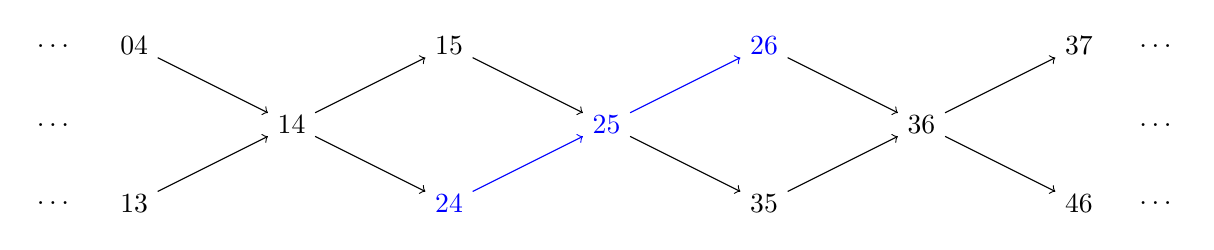
\begin{tikzpicture}

% Nodes for vertices
\node(zca) at (0,0){13};
\node(baz) at (0,2){04};
\node(aba) at (2,1){14};
\node(zcb) at (4,0){\color{blue}{24}};
\node(baa) at (4,2){15};
\node(abb) at (6,1){\color{blue}{25}};
\node(zcc) at (8,0){35};
\node(bab) at (8,2){\color{blue}{26}};
\node(abc) at (10,1){36};
\node(zcd) at (12,0){46};
\node(bac) at (12,2){37};

% Nodes for ellipses
\node at (-1,0){\dots};
\node at (-1,1){\dots};
\node at (-1,2){\dots};

\node at (13,0){\dots};
\node at (13,1){\dots};
\node at (13,2){\dots};

% Drawing arrows
\draw[->] (zca) -- (aba);
\draw[->] (aba) -- (baa);
\draw[->] (baz) -- (aba);
\draw[->] (aba) -- (zcb);
\draw[->] (baa) -- (abb);
\draw[->] (abb) -- (zcc);
\draw[->,blue] (zcb) -- (abb);
\draw[->,blue] (abb) -- (bab);
\draw[->] (bab) -- (abc);
\draw[->] (abc) -- (zcd);
\draw[->] (zcc) -- (abc);
\draw[->] (abc) -- (bac);

\end{tikzpicture}
}
\]
\end{figure}

\begin{figure}
\caption{$\tilde{Q}^{(2, 3)}$, with a slice shown in blue}\label{fig:q23}
\[
\scalebox{0.7}{
\begin{tikzpicture}

% Nodes for vertices

%Layer 0
\node(zzcz) at (0,0){135};
\node(azbz) at (6,0){146};
\node(bzaz) at (12,0){157};
\node(zabz) at (3,1){136};
\node(aaaz) at (9,1){147};
\node(zbaz) at (6,2){137};

% Layer 1
\node(zzca) at (2,3){246};
\node(azba) at (8,3){257};
\node(bzaa) at (14,3){\color{blue}{268}};
\node(zaba) at (5,4){247};
\node(aaaa) at (11,4){\color{blue}{258}};
\node(zbaa) at (8,5){\color{blue}{248}};

% Layer 2
\node(zzcb) at (4,6){\color{blue}{357}};
\node(azbb) at (10,6){\color{blue}{368}};
\node(bzab) at (16,6){379};
\node(zabb) at (7,7){\color{blue}{358}};
\node(aaab) at (13,7){369};
\node(zbab) at (10,8){359};

% Nodes for ellipses
\node at (0,-1){\dots};
\node at (6,-1){\dots};
\node at (12,-1){\dots};

\node at (4,9){\dots};
\node at (10,9){\dots};
\node at (16,9){\dots};

% Drawing arrows

% Layer 0
\draw[->] (zzcz) -- (zabz);
\draw[->] (zabz) -- (azbz);
\draw[->] (azbz) -- (aaaz);
\draw[->] (aaaz) -- (bzaz);
\draw[->] (zabz) -- (zbaz);
\draw[->] (zbaz) -- (aaaz);

% Layer 1
\draw[->] (zzca) -- (zaba);
\draw[->] (zaba) -- (azba);
\draw[->] (azba) -- (aaaa);
\draw[->,blue] (aaaa) -- (bzaa);
\draw[->] (zaba) -- (zbaa);
\draw[->,blue] (zbaa) -- (aaaa);

% Layer 2
\draw[->,blue] (zzcb) -- (zabb);
\draw[->,blue] (zabb) -- (azbb);
\draw[->] (azbb) -- (aaab);
\draw[->] (aaab) -- (bzab);
\draw[->] (zabb) -- (zbab);
\draw[->] (zbab) -- (aaab);

% between layers
\draw[->] (azbz) -- (zzca);
\draw[->] (bzaz) -- (azba);
\draw[->] (aaaz) -- (zaba);

\draw[->] (azba) -- (zzcb);
\draw[->,blue] (bzaa) -- (azbb);
\draw[->,blue] (aaaa) -- (zabb);

\end{tikzpicture}
}
\]
\end{figure}

Following \cite[Definition 5.20]{io}, we define a \emph{slice} of $\tqdn$ to be a full subquiver $S$ of $\tqdn$ such that:
\begin{enumerate}
\item Any $\nu_{d}$ orbit in $\tqdn$ contains precisely one vertex which belongs to $S$.
\item $S$ is convex, i.e., for any path $P$ in $\tqdn$ connecting two vertices in $S$, all vertices appearing in $P$ belong to $S$.
\end{enumerate}
Slices are shown in blue in Figure~\ref{fig:q13} and Figure~\ref{fig:q23}.

Given a slice $S$ of $\tqdn$, one can find a cut $C_{S}$ of $\qdn$ such that $Q_{C_{S}}^{(d, n)}$ is isomorphic to $S$ with the arrows $F_{i}$ of $Q_{C_{S}}^{(d, n)}$ corresponding to arrows $A \to A + E_{i}$ in $S$ \cite[Theorem 5.24]{io}.

\begin{rema}
These combinatorial constructions of course have representation-theoretic interpretations, which are explained in \cite{io}. Cuts and slices correspond to iterated $d$-APR tilts. The map $\nu_{d}$ is the $d$-th desuspension of the Serre functor on the derived category. The map $\pi$ corresponds to the projection from the derived category to the $(d + 2)$-angulated cluster category \cite{ot}.
\end{rema}

\subsubsection{Mutation of cuts and slices}\label{sect:back:cut_slice:mut}

Cuts and slices can be mutated, as was defined in~\cite{io}. This corresponds to algebraic mutation and also to bistellar flips.
\begin{itemize}
\item Let $C$ be a cut of $\qdn$ and let $x$ be a source of $\qdn_{C}$. Define a subset $\mu_{x}^{+}(C)$ of $\qdn_{1}$ by removing all arrows in $C$ which end at $x$ and adding all arrows in $\qdn_{1}$ which begin at $x$. Dually, if $x$ is a sink of $\qdn_{C}$, define $\mu_{x}^{-}(C)$ by removing all arrows in $C$ which begin at $x$ and adding all arrows in $\qdn_{1}$ which end at $x$. By \cite[Proposition 5.14]{io}, we have that $\mu_{x}^{+}(C)$ and $\mu_{x}^{-}(C)$ are also cuts of $\qdn$. This process is illustrated in Figure~\ref{fig:cut_mut}.
\item Let $S$ be a slice of $\tqdn$. If $x$ is a source of $S$, then define a full subquiver $\mu_{x}^{+}(S)$ of $\tqdn$ by removing $x$ from $S$ and adding $\nu_{d}^{-1}x$ \cite[Definition 5.25]{io}. Dually, if $x$ is a sink of $S$, define a full subquiver $\mu_{x}^{-}(S)$ by removing $x$ and adding $\nu_{d}x$. This process is illustrated in Figure~\ref{fig:slice_mut}.
\end{itemize}
If $C_{S}$ is the cut corresponding to a slice $S$ then $C_{\mu_{x}^{+}{S}} = \mu_{x}^{+}(C_{S})$ and $C_{\mu_{x}^{-}{S}} = \mu_{x}^{-}(C_{S})$, provided $x$ is a source or sink, respectively. Here we abuse notation by using $x$ to refer both to the relevant vertex of $S$ and to the relevant vertex of $\qdn_{C_{S}}$.

\begin{figure}
\caption{Mutating the cut of $Q^{(2,3)}$ from Figure~\ref{fig:qdn_cuts} at vertex 101}\label{fig:cut_mut}
\[
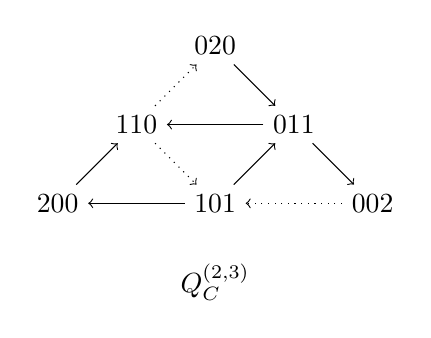
\begin{tikzpicture}

%%%%%%%%%%%%%%%%%%%%%%%%%%
% A_3^2
%%%%%%%%%%%%%%%%%%%%%%%%%%

\begin{scope}[shift={(3,0)}]

\node(200) at (0,0) {200};
\node(110) at (1,1) {110};
\node(020) at (2,2) {020};
\node(011) at (3,1) {011};
\node(002) at (4,0) {002};
\node(101) at (2,0) {101};

\draw[->] (200) -- (110);
\draw[->,dotted] (110) -- (020);
\draw[->] (020) -- (011);
\draw[->] (011) -- (002);
\draw[->,dotted] (002) -- (101);
\draw[->] (101) -- (200);
\draw[->,dotted] (110) -- (101);
\draw[->] (101) -- (011);
\draw[->] (011) -- (110);

\node at (2,-1) {$Q_{C}^{(2,3)}$};

\end{scope}

\end{tikzpicture}
\]
\end{figure}

\begin{figure}
\caption{Mutating the slice from Figure~\ref{fig:q23} at the vertex 368}\label{fig:slice_mut}
\[
\scalebox{0.7}{
\begin{tikzpicture}

% Nodes for vertices

%Layer 0
\node(zzcz) at (0,0){135};
\node(azbz) at (6,0){146};
\node(bzaz) at (12,0){157};
\node(zabz) at (3,1){136};
\node(aaaz) at (9,1){147};
\node(zbaz) at (6,2){137};

% Layer 1
\node(zzca) at (2,3){246};
\node(azba) at (8,3){\color{blue}{257}};
\node(bzaa) at (14,3){\color{blue}{268}};
\node(zaba) at (5,4){247};
\node(aaaa) at (11,4){\color{blue}{258}};
\node(zbaa) at (8,5){\color{blue}{248}};

% Layer 2
\node(zzcb) at (4,6){\color{blue}{357}};
\node(azbb) at (10,6){368};
\node(bzab) at (16,6){379};
\node(zabb) at (7,7){\color{blue}{358}};
\node(aaab) at (13,7){369};
\node(zbab) at (10,8){359};

% Nodes for ellipses
\node at (0,-1){\dots};
\node at (6,-1){\dots};
\node at (12,-1){\dots};

\node at (4,9){\dots};
\node at (10,9){\dots};
\node at (16,9){\dots};

% Drawing arrows

% Layer 0
\draw[->] (zzcz) -- (zabz);
\draw[->] (zabz) -- (azbz);
\draw[->] (azbz) -- (aaaz);
\draw[->] (aaaz) -- (bzaz);
\draw[->] (zabz) -- (zbaz);
\draw[->] (zbaz) -- (aaaz);

% Layer 1
\draw[->] (zzca) -- (zaba);
\draw[->] (zaba) -- (azba);
\draw[->,blue] (azba) -- (aaaa);
\draw[->,blue] (aaaa) -- (bzaa);
\draw[->] (zaba) -- (zbaa);
\draw[->,blue] (zbaa) -- (aaaa);

% Layer 2
\draw[->,blue] (zzcb) -- (zabb);
\draw[->] (zabb) -- (azbb);
\draw[->] (azbb) -- (aaab);
\draw[->] (aaab) -- (bzab);
\draw[->] (zabb) -- (zbab);
\draw[->] (zbab) -- (aaab);

% between layers
\draw[->] (azbz) -- (zzca);
\draw[->] (bzaz) -- (azba);
\draw[->] (aaaz) -- (zaba);

\draw[->,blue] (azba) -- (zzcb);
\draw[->] (bzaa) -- (azbb);
\draw[->,blue] (aaaa) -- (zabb);

\end{tikzpicture}
}
\]
\end{figure}

\section{Triangulations without interior $(d+1)$-simplices}\label{sect:triangs}

In this section we prove our combinatorial description of triangulations of $C(n + 2d + 1, 2d)$ without interior $(d + 1)$-simplices and use this description to show that this class of triangulations is connected by bistellar flips. From the perspective of polyhedral geometry, this provides a combinatorial description of the triangulations without interior $(d + 1)$ and shows how they sit within the class of all triangulations. From the perspective of representation theory, this gives a geometric description of iterated $d$-APR tilts of $A_{n}^{d}$.

\subsection{The quiver of a triangulation}

We first define the quiver of a triangulation, which is the higher-dimensional version of the quiver of a polygon triangulation---see, for instance, \cite[Section 3]{cdm-03} and \cite[Definition 2.12]{lkw-clus-intro}.

\begin{defi}\label{def:quiver}
Given a triangulation $\mathcal{T}$ of $C(n + 2d + 1, 2d)$, we define the \emph{quiver} $Q(\mathcal{T})$ of $\mathcal{T}$ to be the following directed graph. The vertices are \[Q_{0}(\mathcal{T}) = \darcs{\mathcal{T}}.\] The arrows are given by $A \to B$ with $A \neq B$ such that $(A - \onevec) \swr B$ and there exists no $A' \in \darcs{\mathcal{T}}\setminus\{A, B\}$ with $(A - \onevec) \swr A'$ and $(A' - \onevec) \swr B$. Recall our convention of taking $A - \onevec$ modulo $n + 2d + 1$.
\end{defi}

We define the quiver in this way so that it coincides with the Gabriel quiver of the endmorphism algebra of the cluster-tilting object corresponding to the triangulation. The arrows mirror the description of the homomorphisms in the cluster category $\mathcal{O}_{A_{n}^{d}}$ from \cite{ot}. However, we now prove a simpler description of the quiver, given in Corollary~\ref{cor:quiv_desc}. In order to obtain this, we first make some observations about cyclic polytopes. Changing the ordering on on $[n + 2d + 1]$ from $<_{1}$ to $<_{l}$ induces a (combinatorial) automorphism of the cyclic polytope $C(n + 2d + 1, 2d)$; see \cite{kw}. We think of this automorphism as reorienting the cyclic polytope. Generalising \cite{ot}, given a $2d$-simplex $T$ of $C(n + 2d + 1,2d)$ and an ordering $<_{l}$ of $[n + 2d + 1]$ under which $T$ is ordered $T = (t_{0}, t_{1}, \dots , t_{2d})$, we write $e_{l}(T) = (t_{0}, t_{2}, \dots , t_{2d-2}, t_{2d})$. If the ordering is determined by the context, we simply write $e(T)$.

\begin{lemma}\label{lem:find_2d_simplex}
Given an ordering $<_{l}$ of $[n + 2d + 1]$ and a $d$-arc $A$ of a triangulation $\mathcal{T}$ of $C(n + 2d + 1,2d)$, there is a $2d$-simplex $T$ of $\mathcal{T}$ such that $e_{l}(T) = A$.
\end{lemma}
\begin{proof}
This follows from applying \cite[Proposition 2.13]{ot} in the orientation given by~$<_{l}$.
\end{proof}

\begin{prop}\label{prop:all_but_one_vertex}
Suppose that $A \rightarrow B$ is an arrow in $Q(\mathcal{T})$. Then $A$ and $B$ share all but one entry, and there is a $2d$-simplex $T$ of $\mathcal{T}$ such that $A$ and $B$ are both faces of $T$.
\end{prop}
\begin{proof}
We have that $(A - \onevec) \swr B$. It must be the case that $A$ and $B$ have at least one common entry, otherwise $A \swr B$. Hence, by re-ordering, we may assume that $a_{0} = b_{0}$ and $a_{d - 1} < a_{d} < b_{d}$. There must be a $2d$-simplex $T$ of $\mathcal{T}$ such that $e(T) = B$. We label the vertices of $T$ by $T = (b_{0}, x_{1}, b_{1}, x_{2}, \dots, b_{d - 1}, x_{d}, b_{d})$.

\sloppy We cannot have that $b_{i - 1} < x_{i} \leq a_{i} - 1$ for all $i \in [d]$, otherwise $A \swr (x_{1}, x_{2}, \dots, x_{d}, b_{d})$, which is impossible since $A$ and $(x_{1}, x_{2}, \dots, x_{d}, b_{d})$ are both $d$-arcs of $\mathcal{T}$. Hence there is an $i \in [d]$ such that $b_{i - 1} < a_{i} - 1 < x_{i}$. Then $(b_{0}, b_{1}, \dots, b_{i - 1}, x_{i}, b_{i + 1}, b_{i + 2}, \dots, b_{d})$ is a $d$-arc of $\mathcal{T}$, since $b_{i - 1} < a_{i} - 1 < x_{i}$ and $x_{i} < b_{i} < b_{i + 1}$. Moreover, $(A - \onevec) \swr (b_{0}, b_{1}, \dots, b_{i - 1}, x_{i}, b_{i + 1}, b_{i + 2}, \dots, b_{d})$ and $(b_{0} - 1, \dots, b_{i - 1} - 1, x_{i} - 1, b_{i + 1} - 1, \dots, b_{d} - 1) \swr B$. Since $A \rightarrow B$ is an arrow in $Q(\mathcal{T})$, we must have $A = (b_{0}, b_{1}, \dots, b_{i - 1}, x_{i}, b_{i + 1}, b_{i + 2}, \dots, b_{d})$. (In fact, by the ordering we have chosen, we must have that $i = d$.) Therefore $A$ and $B$ are both faces of the $2d$-simplex $T$ and they share all but one entry, as desired.
\end{proof}

\begin{coro}\label{cor:quiv_desc}
The arrows of $Q(\mathcal{T})$ are \[Q_{1}(\mathcal{T}) = \set{A \rightarrow A + \rvec \st \parbox{6.5cm}{\begin{center}$A, A + \rvec \in \nonconsec{n + 2d + 1}{d},$ $\nexists s \in [r - 1] \text{ such that } A + \svec \in Q_{0}(\mathcal{T})$\end{center}}}.\]
\end{coro}

We call arrows $A \to A + \rvec$ \emph{arrows of type $i$}, analogously to our terminology of arrows of type~$i$ in $\qdn$ from Section~\ref{sect:back:cut_slice}. Note that this labelling depends on the choice of an ordering $<_{l}$.

For an arrow $\alpha$, we denote the \emph{head} $h(\alpha)$ and the \emph{tail} $t(\alpha)$ such that $t(\alpha) \xrightarrow{\alpha} h(\alpha)$. We say that $\alpha$ is \emph{incident} at $t(\alpha)$ and $h(\alpha)$. Given a quiver $Q$ with vertices $A,B \in Q_{0}$, by a \emph{path} in $Q$ from $A$ to $B$ we mean a finite sequence of arrows $\alpha_{1}\dots\alpha_{r}$ such that $t(\alpha_{1}) = A, h(\alpha_{r}) = B$ and $h(\alpha_{i - 1}) = t(\alpha_{i})$ for all $i \in \{2, 3, \dots, s\}$. If there is a path from $A$ to $B$, then we write $A \leadsto B$. We note the following property concerning paths in $Q(\mathcal{T})$ which will be useful later.

\begin{lemma}\label{lem:find_path}
Given a triangulation $\mathcal{T}$ of $C(n + 2d + 1, 2d)$ and $A, B \in Q_{0}(\mathcal{T})$ with $(A - \onevec) \swr B$, there is a path from $A$ to $B$ in $Q(\mathcal{T})$.
\end{lemma}
\begin{proof}
This is clear from Definition~\ref{def:quiver}, using induction.
\end{proof}

\subsection{Quiver description}\label{sect:main}

With these preliminaries taken care of, we now move to prove the first main result of this paper, which describes triangulations $\mathcal{T}$ without interior $(d + 1)$-simplices in terms of their quivers $Q(\mathcal{T})$. Recall that a $(d + 1)$-simplex of a triangulation $\mathcal{T}$ of $C(n + 2d + 1, 2d)$ is interior if all of its facets are $d$-arcs.

Slices of $\tqdn$ give triangulations of $C(n + 2d + 1, 2d)$. We give a direct combinatorial proof of this, although it can also be deduced from the fact that slices correspond to iterated $d$-APR tilts \cite[Theorem 4.15]{io}, which implies that projecting to the cluster category will give a triangulation \cite[Theorem 6.4]{ot}. Recall the map $\pi$ from Definition~\ref{def:pi}.

\begin{prop}\label{prop:slice->triang}
If $S$ is a slice of $\tqdn$, then the vertices $\pi(S_{0})$ give a triangulation of $C(n + 2d + 1, 2d)$.
\end{prop}
\begin{proof}
There are as many $\nu_{d}$-orbits as there are elements of $\nonconsec{n + 2d + 1}{d}$ containing $1$, namely $\binom{n + d - 1}{d}$. Suppose that there exist $\pi(A)$ and $\pi(B)$ in $\pi(S_{0})$ with $\pi(A) \swr \pi(B)$. We assume without loss of generality that $a_{0} < b_{0}$, noting that $\pi(A) \swr \pi(B)$ implies that $a_{i} \neq b_{i}$ for all $i$. We claim that $A < B$. Suppose for contradiction that $b_{i} < a_{i}$ for some $i$. We may choose the minimal $i$ such that this is the case. Then $a_{i - 1} < b_{i - 1} < b_{i} < a_{i}$. Since we must have \[\pi(a_{i - 1}) < \pi(b_{i - 1}) < \pi(a_{i}) < \pi(b_{i}),\] we must have $a_{i} - a_{i - 1} > n + 2d + 1$. Hence $a_{d} - a_{0} > n + 2d + 1 > n + 2d - 1$, which contradicts $A \in \derset{n + 2d + 1}{d}$.

Therefore $A < A + \onevec \leqslant B$, which means that here is then a path $A \leadsto A + \onevec \leadsto B$, so $A + \onevec \in \pi(S_{0})$ by convexity. But this contradicts the fact that $S$ contains one vertex from every $\nu_{d}$-orbit. Hence $\pi(S_{0})$ is a non-intertwining subset of $\nonconsec{n + 2d + 1}{d}$ of size $\binom{n + d - 1}{d}$, and so gives a triangulation of $C(n + 2d + 1, 2d)$.
\end{proof}

A similar argument also shows the following lemma, which will be useful later.

\begin{lemma}\label{lem:conv->slice}
If $S$ is a convex subquiver of $\tqdn$ such that $\pi(S_{0})$ is a triangulation of $C(n+2d+1,2d)$, then $S$ is a slice. 
\end{lemma}
\begin{proof}
Suppose that $S$ is a convex subquiver such that $\pi(S_{0})$ is a triangulation of $C(n + 2d + 1, 2d)$. Suppose for contradiction that $S$ possesses two vertices $A$ and $B$ which are in the same $\nu_{d}$-orbit. There is then either a path $A \leadsto B$ or a path $B \leadsto A$. Without loss of generality, we suppose the former. But then there is a path $A \leadsto A + \onevec \leadsto B$, so we must have $A + \onevec \in S_{0}$ by convexity. This is a contradiction, since $\pi(A)$ and $\pi(A + \onevec)$ are intertwining.
\end{proof}

The main theorem of this section is as follows. This shows how the quivers of triangulations detect the structure of the triangulation, and gives a geometric description of iterated $d$-APR tilts of $A_{n}^{d}$.

\begin{theorem}\label{thm:interior}
A triangulation $\mathcal{T}$ of $C(n + 2d + 1, 2d)$ has no interior $(d+1)$-simplices if and only if its quiver is a cut of $\qdn$, and this is the case if and only if its quiver has no cycle.
\end{theorem}

Our strategy for proving this theorem is to prove facts about the quivers $Q(\mathcal{T})$ for triangulations $\mathcal{T}$ of $C(n + 2d + 1, 2d)$ without internal $(d + 1)$-simplices. We then use these properties to show that one can realise $Q(\mathcal{T})$ as a slice of $\tqdn$, which will imply that $Q(\mathcal{T})$ is a cut of $\qdn$. The idea of the proofs of both of the following lemmas is that if $Q(\mathcal{T})$ does not possess a certain property, then we can find an interior $(d + 1)$-simplex in~$\mathcal{T}$.

\begin{lemma}\label{lem:single-step-arrows}
If $\mathcal{T}$ has no interior $(d+1)$-simplices, then the arrows in $Q(\mathcal{T})$ are all of the form $A \rightarrow A + E_{i}$.
\end{lemma}
\begin{proof}
By Proposition~\ref{prop:all_but_one_vertex}, every arrow is of the form $A \rightarrow A + \rvec$ for some $r>0$ and for each such arrow, we have that $(a_{0}, a_{1}, \dots, a_{i}, a_{i} + r, a_{i+1}, a_{i + 2}, \dots, a_{d})$ is a face of a $2d$-simplex of $\mathcal{T}$. If $r>1$, then this is an interior $(d+1)$-simplex.
\end{proof}

\begin{lemma}\label{lem:simp_arrow_switch}
Suppose that $\mathcal{T}$ has no interior $(d+1)$-simplices. If $A \rightarrow A + E_{i} \rightarrow A + E_{i} + E_{j}$ is a sequence of arrows in $Q(\mathcal{T})$, then, if $A + E_{j} \in \nonconsec{n+2d+1}{d}$, the sequence $A \rightarrow A + E_{j} \rightarrow A + E_{i} + E_{j}$ is also in $Q(\mathcal{T})$.
\end{lemma}
\begin{proof}
We assume $A + E_{j} \in \nonconsec{n+2d+1}{d}$. By re-ordering, we may assume that $i = d$. Then there is a $2d$-simplex $T$ of $\mathcal{T}$ such that $e(T) = A + E_{j} + E_{d}$ by Lemma~\ref{lem:find_2d_simplex}.

Let $T = (a_{0}, x_{1}, a_{1}, \dots, x_{j}, a_{j} + 1, x_{j + 1}, \dots, x_{d}, a_{d} + 1)$. If $x_{d} = a_{d}$, then $A + E_{j}$ is a $d$-face of $T$ and hence a $d$-arc of $\mathcal{T}$. Hence, suppose for contradiction that $a_{d} \neq x_{d}$, so that $a_{d - 1} < x_{d} \leqslant a_{d} - 1$. Note that if $x_{j} = a_{j - 1} + 1$, then $(a_{0}, a_{1}, \dots , a_{d}) \swr (x_{1}, x_{2}, \dots ,x_{d}, a_{d} + 1)$, which is a $d$-face of $T$. Hence $a_{j - 1} + 2 \leqslant x_{j} < a_{j} + 1$. Then $(a_{0}, a_{1}, \dots, a_{j - 1}, x_{j}, x_{j + 1}, \dots , x_{d}, a_{d} + 1)$ is a $(d + 1)$-face of $T$ and an interior $(d+1)$-simplex of $\mathcal{T}$, a contradiction.
\end{proof}

We now prove some facts about the quivers $\tqdn$, which will be useful in proving the main theorem of this section. These will be used in combination with the previous two lemmas to show that one can realise $\mathcal{Q}(\mathcal{T})$ as a slice if $\mathcal{T}$ has no interior $(d + 1)$-simplices. We say that a full subquiver $P$ of $\tqdn$ is \emph{switching-closed} if whenever $A \rightarrow A + E_{i} \rightarrow A + E_{i} + E_{j}$ is a sequence of arrows in $P$ and $A + E_{j} \in \tqdn_{0}$, then the sequence of arrows $A \rightarrow A + E_{j} \rightarrow A + E_{i} + E_{j}$ is also in $P$.

\begin{lemma}\label{lem:all_paths}
Let $P$ be a switching-closed full subquiver of $\tqdn$. If there is a path $A \leadsto B$ in $P$, all other paths $A \leadsto B$ in $\tqdn$ must also lie in $P$.
\end{lemma}
\begin{proof}
Suppose that we have a path $A \leadsto B$ in $P$. The length of any such path is $\sum_{i = 0}^{d}(b_{i} - a_{i})$. We prove the claim by induction on this quantity. The base case, where the length is $1$, follows from the fact that $P$ is a full subquiver of $\tqdn$.

For the inductive step, we assume that the claim holds for all $X$ and $Y$ with $\sum_{i = 0}^{d}(y_{i} - x_{i}) < \sum_{i = 0}^{d}(b_{i} - a_{i})$. We have that $B$ is the head of up to $(d + 1)$ arrows, namely the ones with tails $B - E_{0}, B - E_{1}, \dots, B - E_{d}$, provided these are vertices of $\tqdn$. Suppose that $B - E_{i}$ is the penultimate vertex of our path $A \leadsto B$.

Choose a vertex $B - E_{j} \in \tqdn_{0}$, where $i \neq j$. If $A \not\leqslant B - E_{j}$, then we may ignore this vertex, since there can be no paths from $A$ to $B$ through it. Hence we assume that $A \leqslant B - E_{j}$. This implies that $A \leqslant B - E_{i} - E_{j} \leqslant B - E_{i}$, so $B - E_{i} - E_{j} \in P_{0}$ by the induction hypothesis applied to $A$ and $B - E_{i}$.

Since $P$ is switching-closed, we have that $B - E_{j} \in P_{0}$, since $B - E_{i} - E_{j}, B - E_{i}, B \in P_{0}$. By the induction hypothesis, all paths $A \leadsto B - E_{j}$ lie in $P$, and hence all paths $A \leadsto B$ passing through $B - E_{j}$ lie in $P$. The result follows.
\end{proof}

By a \emph{walk} in a quiver $Q$ from $A$ to $B$ we mean a finite sequence of arrows $\beta_{1}\beta_{2}\dots\beta_{s}$ such that $\beta_{1}$ is incident at $A$, $\beta_{s}$ is incident at $B$, and $\beta_{i-1}$ and $\beta_{i}$ are incident at a common vertex for all $i \in \{2, 3, \dots, s\}$. In this case, we write $A \walk B$. That is, a path only consists of forwards arrows, but a walk may contain backwards arrows as well.

\begin{lemma}\label{lem:walk_to_path}
Let $P$ be a connected switching-closed full subquiver of $\tqdn$. If $A,B \in P_{0}$ are such that there is a path $A \leadsto B$ in $\tqdn$, then there is a path $A \leadsto B$ in $P$.
\end{lemma}
\begin{proof}
Let $A,B \in P_{0}$. Suppose that there is a path $A \leadsto B$ in $\tqdn$. There is certainly a walk $W \colon A \walk B$ in $P$, since $P$ is connected. We prove that there is also a path $A \leadsto B$ in $P$ by induction on the number of backwards arrows in this walk. The base case, in which there are zero backwards arrows in the walk, is immediate.

Hence we suppose for induction that the claim holds for walks with fewer backwards arrows than $W$. We may assume that the final arrow in $W$ is a backwards one, otherwise we may remove the final arrow and consider instead the walk $A \walk B'$, where $A \walk B' \rightarrow B$ is the original walk~$W$.

Therefore we can assume that our walk is of the form $A \walk C \leftarrow B$, where $C \in P$. By the induction hypothesis, we can replace this with a walk of the form $A \leadsto C \leftarrow B$ in $P$. Moreover, by Lemma~\ref{lem:all_paths} we have that all paths $A \leadsto C$ in $\tqdn$ lie in $P$. Since we have a path $A \leadsto B$ in $\tqdn$, we have $A \leqslant B$ and, moreover, $A \leqslant B \leqslant C$. There is therefore a path $A \leadsto B \leadsto C$ in $\tqdn$. This path is in $P$, since every path $A \leadsto C$ is in $P$, which gives the desired path $A \leadsto B$ in~$P$.
\end{proof}

These two lemmas imply the following corollary.

\begin{coro}\label{cor:switch+con->conv}
Let $P$ be a connected switching-closed full subquiver of $\tqdn$. Then $P$ is convex in $\tqdn$.
\end{coro}
\begin{proof}
Suppose that $P$ is a connected switching-closed full subquiver of $\tqdn$. Let $A, B \in P_{0}$ be such that there is a path $A \leadsto B$ in $\tqdn$. By Lemma~\ref{lem:walk_to_path}, there is a path $A \leadsto B$ in $P$. Then, by Lemma~\ref{lem:all_paths}, we have that all paths $A \leadsto B$ lie in $P$, and so $P$ is convex.
\end{proof}

This corollary is useful because it is easier to check the property of being connected and switching-closed than the property of being convex. Given a full subquiver $P$ of $\tqdn$, we write $\overline{P}$ for the smallest switching-closed subquiver containing $P$. The subquiver $\overline{P}$ is well-defined since the intersection of a set of switching-closed full subquivers is switching-closed, so $\overline{P}$ may be constructed as the intersection of all switching-closed subquivers containing $P$.

\begin{prop}\label{prop:no-cyc}
A triangulation $\mathcal{T}$ contains an interior $(d+1)$-simplex if and only if $Q(\mathcal{T})$ contains a cycle.
\end{prop}
\begin{proof}
We first suppose for contradiction that $\mathcal{T}$ contains no interior $(d+1)$-simplices and that $Q(\mathcal{T})$ does contain a cycle. By Lemma~\ref{lem:single-step-arrows}, we can realise this cycle as a path $P \colon A \leadsto B$ in $\tqdn$, where $A$ is some vertex in the cycle in $Q(\mathcal{T})$ and $\pi(B) = A$ with $A \neq B$. We consider this path $P$ as a subquiver of $\tqdn$. By Lemma~\ref{lem:all_paths}, every path $A \leadsto B$ in $\tqdn$ must lie in $\overline{P}$. There is a path $A \leadsto A + \onevec \leadsto B$ in $\tqdn$. Hence $A + \onevec$ is a vertex of $\overline{P}$. By Lemma~\ref{lem:simp_arrow_switch}, if $C$ is a vertex of $\overline{P}$, then $\pi(C)$ is a vertex of $Q(\mathcal{T})$. Therefore $\pi(A + \onevec)$ is a vertex of $Q(\mathcal{T})$, but this is a contradiction, since $\pi(A + \onevec)$ and $A$ are intertwining.

We now suppose that $\mathcal{T}$ is a triangulation with an interior $(d + 1)$-simplex  $(a_{0}, \dots, a_{d + 1})$. Then $Q(\mathcal{T)}$ has a cycle given by concatenating the paths
\begin{align*}
(a_{0}, a_{1}, \dots, a_{d - 1}, a_{d}) &\leadsto (a_{0}, a_{1}, \dots , a_{d - 1}, a_{d + 1}) \leadsto (a_{0}, a_{1}, \dots, a_{d - 2}, a_{d}, a_{d + 1}) \leadsto \\
 \dots &\leadsto (a_{1}, a_{2}, \dots, a_{d}, a_{d + 1}) \leadsto (a_{0}, a_{1}, \dots , a_{d}),
\end{align*}
noting Lemma~\ref{lem:find_path}.
\end{proof}

\begin{rema}
For $d = 1$, an interior triangle gives a 3-cycle in the quiver where all the vertices of the cycle are edges of the triangle. For $d > 1$, the cycle obtained in Proposition~\ref{prop:no-cyc} may not exclusively have facets of the interior $(d + 1)$-simplex as its vertices. An example of this can be seen in Figure~\ref{fig:cyc_triang}, where the interior 3-simplex is 1357, but the cycle is $135 \to 136 \to 137 \to 147 \to 157 \to 357 \to 135$. Here $136$ and $147$ are not faces of the interior 3-simplex 1357.
\end{rema}

We are now ready to prove our first main result, noting that the second part of the statement has already been established by Proposition~\ref{prop:no-cyc}.

\begin{proof}[Proof of Theorem~\ref{thm:interior}]
First suppose that $\mathcal{T}$ has no interior $(d+1)$-simplices. We consider the full subquiver $R$ of $\tqdn$ with vertices \[R_{0} = \set{ B \in \tqdn_{0} \st \pi(B) \in Q_{0}(\mathcal{T})}.\] We claim that this is disconnected and that each connected component gives $Q(\mathcal{T})$ by applying $\pi$. Let $A \in Q_{0}(\mathcal{T})$. If $R$ is connected then it contains a walk $W \colon A \walk (a_{1}, a_{2}, \dots, a_{d}, a_{0} + n + 2d + 1)$. We consider $W$ as a subquiver of $\tqdn$ and consider~$\overline{W}$. By Lemma~\ref{lem:walk_to_path}, $\overline{W}$ contains a path $P \colon A \leadsto (a_{1}, a_{2}, \dots, a_{d}, a_{0} + n + 2d + 1)$. By Lemma~\ref{lem:simp_arrow_switch}, if $B$ is a vertex of $\overline{W}$, then $\pi(B)$ is a vertex of $Q(\mathcal{T})$. Hence all vertices of $P$ give vertices of $Q(\mathcal{T})$, which therefore contains a cycle. But this contradicts Proposition~\ref{prop:no-cyc}.

By this argument, $R$ is disconnected and, moreover, the vertices of each connected component are in bijection with the vertices of $Q(\mathcal{T})$ via $\pi$, since $Q(\mathcal{T})$ is connected. Moreover, the arrows in each connected component of $R$ are the same as the arrows in $Q(\mathcal{T})$, by Lemma~\ref{lem:single-step-arrows}. Hence, by choosing one of the connected components, we obtain a full subquiver $S$ of $\tqdn$ such that $\pi(S) = Q(\mathcal{T})$. We then have that $S$ is a switching-closed connected subquiver of $\tqdn$, so $S$ is convex by Lemma~\ref{cor:switch+con->conv}. Since $\pi(S_{0})$ is a triangulation, it then follows from Lemma~\ref{lem:conv->slice} that $S$ is a slice. Hence $Q(\mathcal{T})$ is a cut of $\qdn$ by \cite[Theorem 5.24]{io}.

Now suppose that $Q(\mathcal{T})$ is a cut of $\qdn$. Then $Q(\mathcal{T})$ cannot contain any cycles, since cut quivers can be realised as slices, which are full subquivers of $\tqdn$, which does not contain any cycles. Then we obtain that $\mathcal{T}$ contains no interior $(d + 1)$-simplices by Proposition~\ref{prop:no-cyc}.
\end{proof}
